\let\negmedspace\undefined
\let\negthickspace\undefined
\documentclass[journal,12pt,twocolumn]{IEEEtran}
\usepackage{gensymb}
\usepackage{amssymb}
\usepackage[cmex10]{amsmath}
\usepackage{amsthm}
\usepackage[export]{adjustbox}
\usepackage{bm}
\usepackage{longtable}
\usepackage{enumitem}
\usepackage{mathtools}
 \usepackage{tikz}
\usepackage[breaklinks=true]{hyperref}
\usepackage{listings}
\usepackage{color}                                            %%
\usepackage{array}                                            %%
\usepackage{longtable}                                        %%
\usepackage{calc}                                             %%
\usepackage{multirow}                                         %%
\usepackage{hhline}                                           %%
\usepackage{ifthen}                                           %%
\usepackage{lscape}     
\usepackage{multicol}
% \usepackage{enumerate}
\DeclareMathOperator*{\Res}{Res}
\renewcommand\thesection{\arabic{section}}
\renewcommand\thesubsection{\thesection.\arabic{subsection}}
\renewcommand\thesubsubsection{\thesubsection.\arabic{subsubsection}}
\renewcommand\thesectiondis{\arabic{section}}
\renewcommand\thesubsectiondis{\thesectiondis.\arabic{subsection}}
\renewcommand\thesubsubsectiondis{\thesubsectiondis.\arabic{subsubsection}}
\hyphenation{op-tical net-works semi-conduc-tor}
\def\inputGnumericTable{}                                 %%
\lstset{
frame=single, 
breaklines=true,
columns=fullflexible
}
\begin{document}

\raggedbottom
\setlength{\parindent}{0pt}
\vspace{3cm}
\title{AI1110-Assignment 1}
\author{Vedant Bhandare\\CS21BTECH11007}
\maketitle
\newpage
\bigskip
\renewcommand{\thefigure}{\theenumi}
\renewcommand{\thetable}{\theenumi}

\section*{\underline{\textbf{Question}}}
The circumference of the base of a cylindrical vessel is 132 cm and its height is 25 cm. Find the

\begin{enumerate}
    \item radius of the cylinder
    \item volume of cylinder.(use $\pi = \frac{22}{7}$)
\end{enumerate}
\section*{\underline{\textbf{Solution}}}
Let $r$ and $h$ be the radius of the base and height of the cylindrical vessel, respectively.\\
Let $C_{base}$ be its base circumference and $V$ be its volume.\\

We know that,

\begin{align}
    C_{base} = 2\pi{r}\\
    V = \pi{r^2h}
\end{align}

\subsection*{\underline{\textbf{1. Radius of the cylinder}}}
\vspace{2mm}
\large{$C_{base} = 2\pi{r}$\hspace{5.25cm}....(1)}
\newline
$132 = 2\pi{r}$
\newline
$132 = 2\times\frac{22}{7}\times{r}$
\newline
$r = 21$
\begin{center}
    Thus the radius of base of the cylindrical vessel is $21 \hspace{1mm}cm$.
\end{center}
\newline
\subsection*{\underline{\textbf{2. Volume of the cylinder}}}
\newline
$V = \pi{r^2h}\hspace{5.25cm}....(2)$
\newline
$V = \frac{22}{7}\times21^2\times25$
\newline
$V = 34650$
\vspace{1mm}
\begin{center}
    {Thus, the volume of the cylindrical vessel is $34650 \hspace{1mm} cm^3.$}
\end{center}
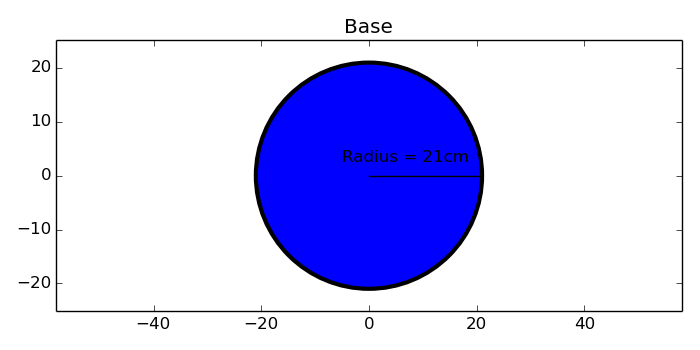
\includegraphics[width = \columnwidth]{Figures/Base.png}
\begin{center}
Base of the cylindrical vessel with radius 21 cm
\end{center}
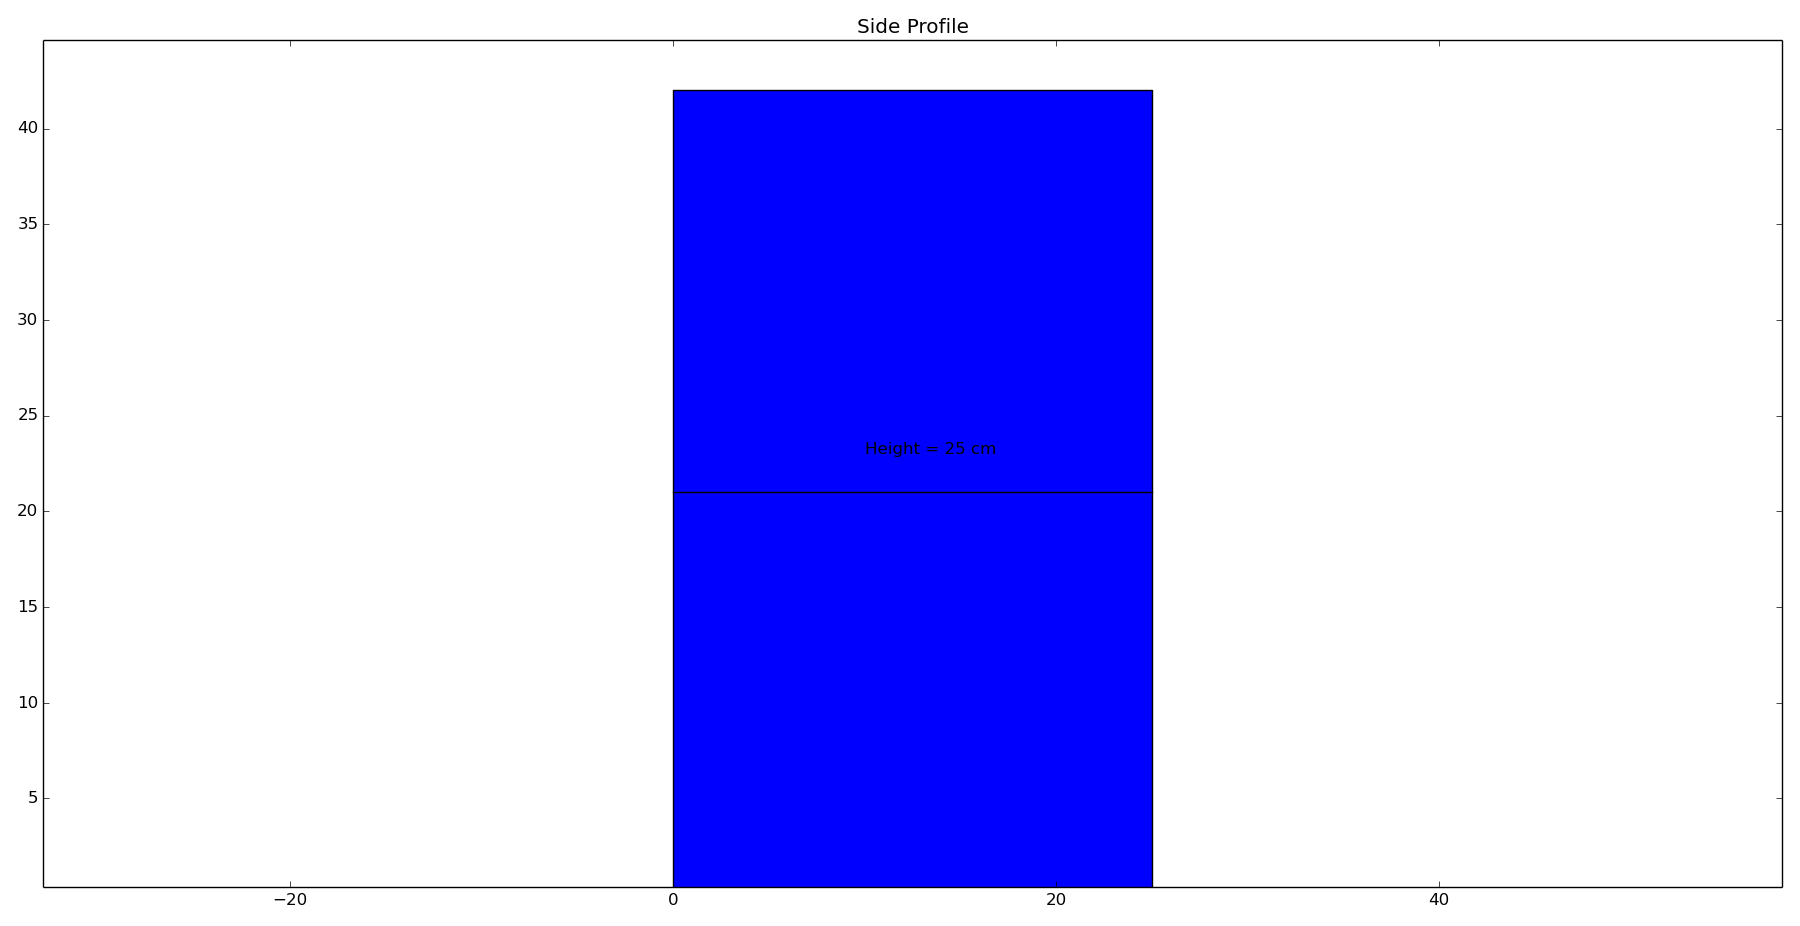
\includegraphics[width = \columnwidth]{Figures/Side Profile.png}
\begin{center}
Side view of the cylindrical vessel with height 25 cm
\end{center}
\end{document}